\subsection{How many Factors?} \label{section:nfactors}
\noindent I follow \citet{guttman1954some} and elect the lower bound of the number of factors based on a simple rule of thumb. The steps are the following.
\begin{enumerate}
\item Calculate the absolute value of the eigenvalues of the correlation matrix of the measurement system.
\item Count the number of eigenvalues greater or equal than one.
\item Define the lower bound of the number of factors as the number of eigenvalues greater than one.
\end{enumerate} 

\indent Once the lower bound is defined, as many eigenvalues as independent measures in the measurement system may be calculated. These are the inputs of the \textit{subjective scree test}. The scree test is an eye ball test of a scatter in which the abscissas are the factor numbers and the ordinates are their corresponding eigenvalues. The lower bound of the number of factors is the actual number of factors if the plot shows a very clear pattern differentiating the factors with eigenvalues greater or equal than one from the rest. In Figure \ref{fig:scree} the lower bound of the number of factors and the actual number of factors are the same according to my criterion because the factors with eigenvalues less than one follow a different pattern from the rest. 

\begin{figure}[H]
	\caption{A Scree Test where the Lower Bound and the Current Number of Factors Agree} \label{fig:scree}
  	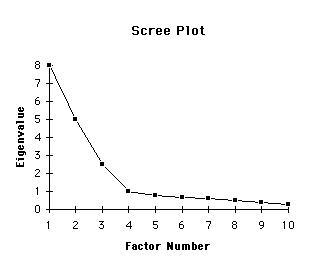
\includegraphics[width=2in, height=2in]{screetest.png}
\end{figure}